\documentclass{article}

\usepackage{graphicx}
\usepackage{tikz}
\usepackage{tikzsymbols}
\usetikzlibrary{calc,patterns,shapes.geometric}
\pagestyle{empty}
\usepackage[margin=0pt]{geometry}
\geometry{papersize={14in,12in}}

\def\centerarc[#1](#2)(#3:#4:#5){\draw[#1] ($(#2)+({#5*cos(#3)},{#5*sin(#3)})$) arc (#3:#4:#5);}

\begin{document}
	\begin{figure}
		\centering
		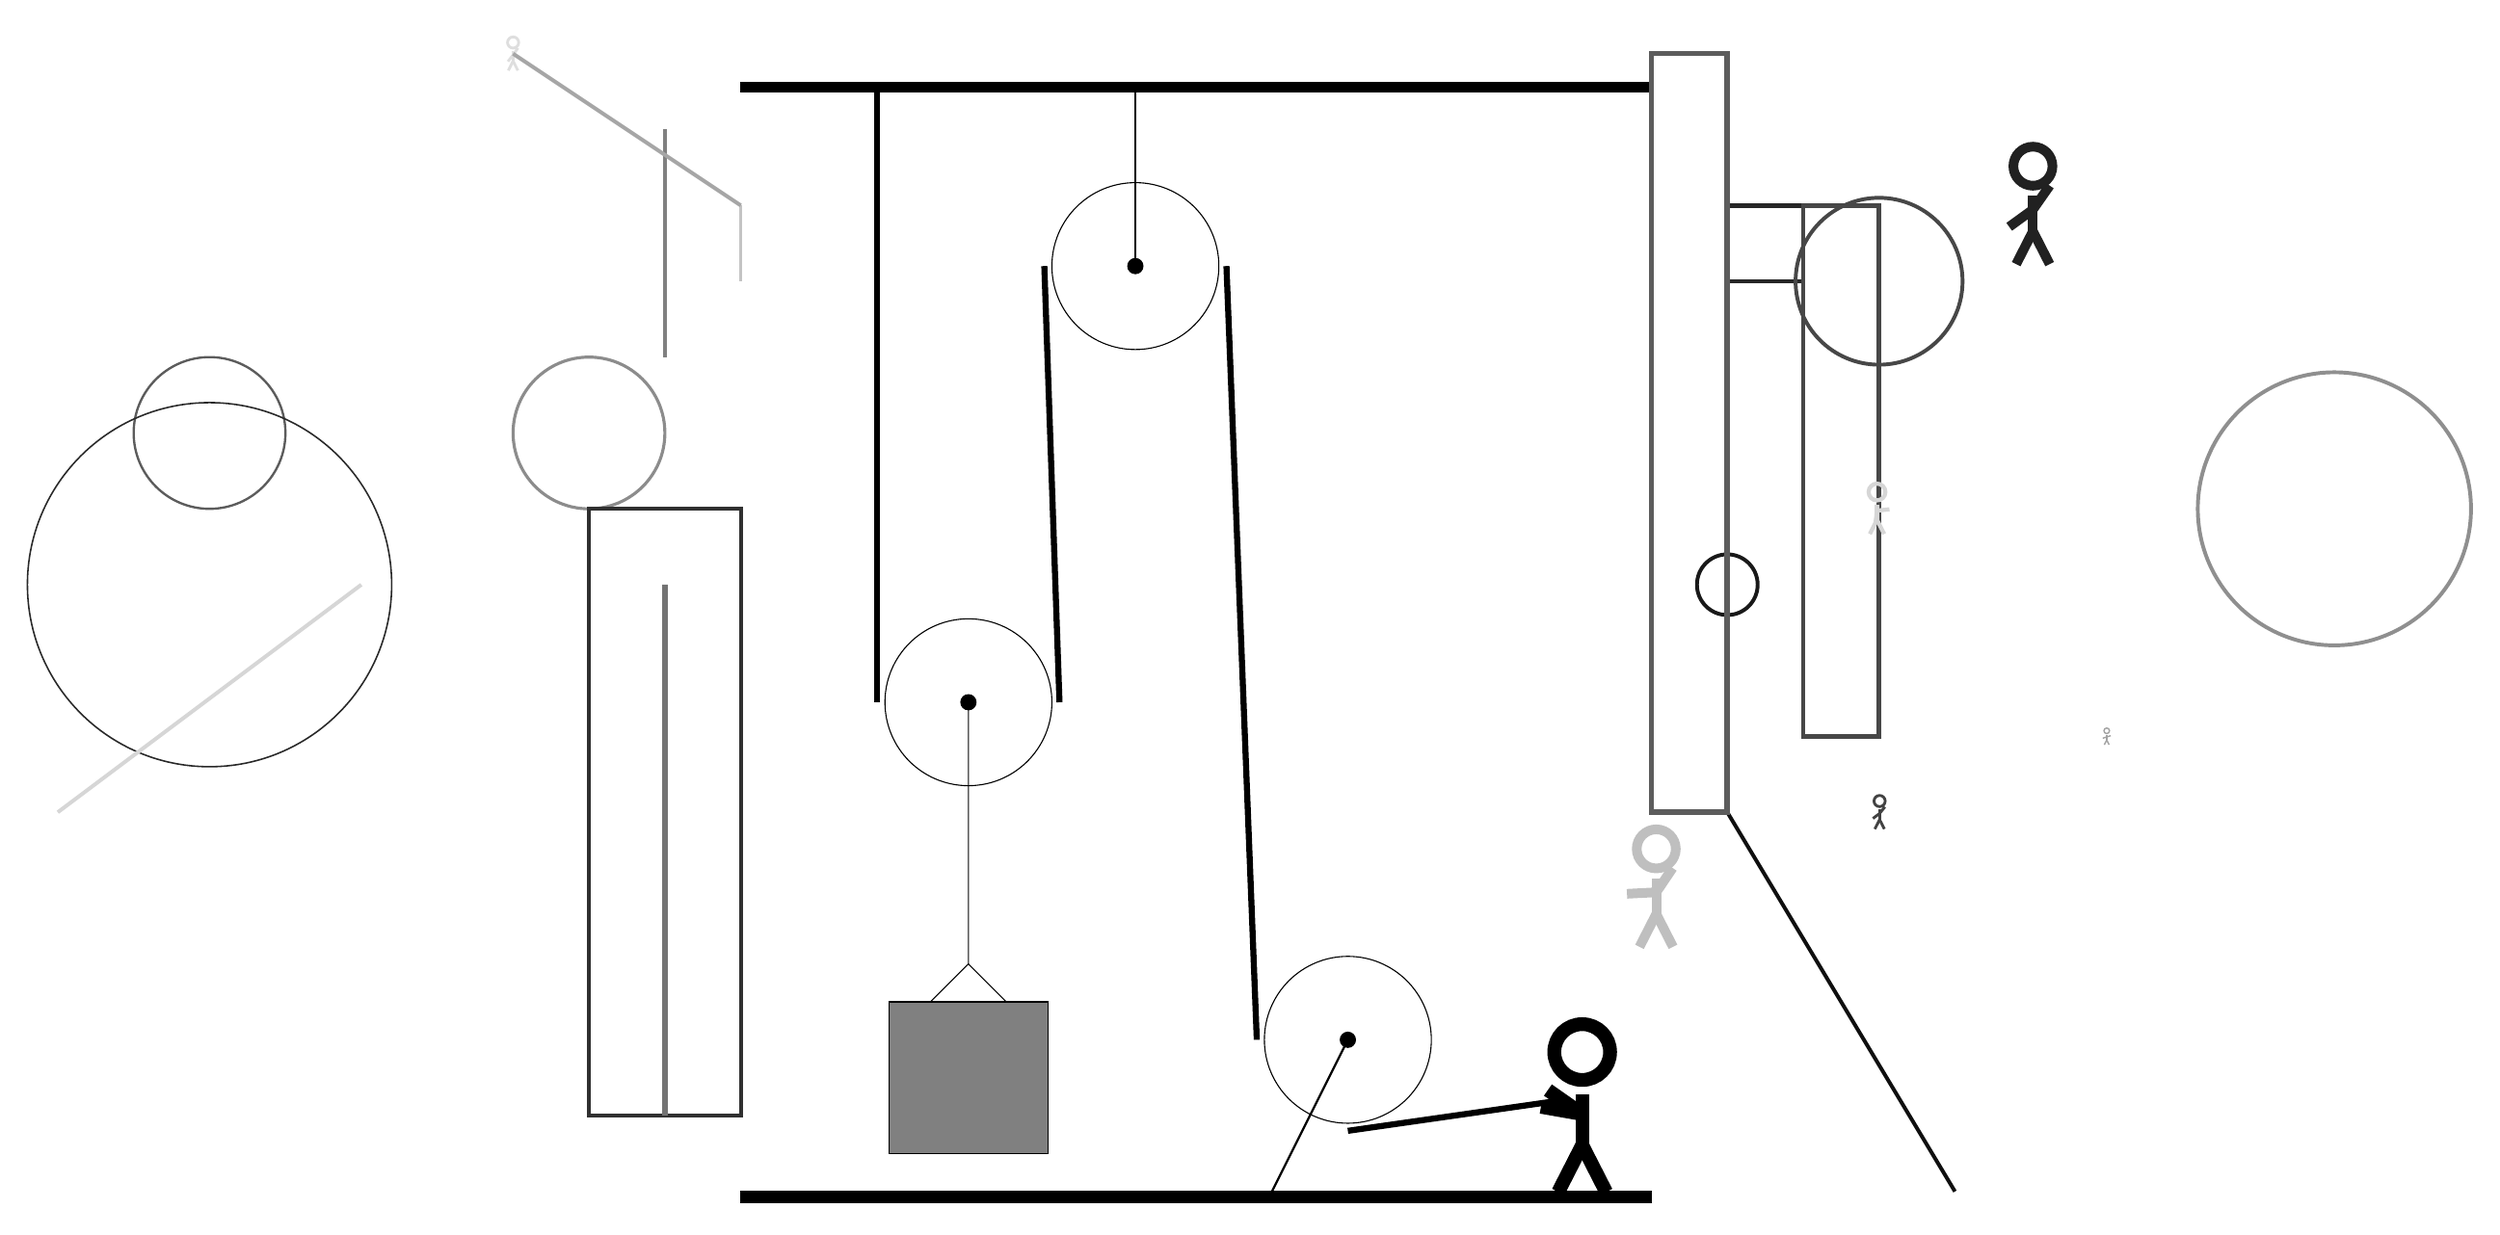
\begin{tikzpicture}
			%%%%% START %%%%%
			
			\draw[fill=black] (-2, 11.5) rectangle (10, 11.625);
			
			\draw (3.2, 9.2) circle (1.1);
			\draw[fill=black] (3.2, 9.2) circle (0.1);
			\draw[thick] (3.2, 9.2) -- (3.2, 11.5);
			
			\draw[line width=0.5mm, color=black!94](11, 2) -- (14, -3);
			
			\draw[line width=0.3mm, color=black!23] (-2, 9) rectangle (-2, 10);
			\draw[line width=0.6mm, color=black!85] (11, 9) rectangle (12, 10);
			\node[line width=0.6mm, color=black!74] at (13, 2) {\Strichmaxerl[2][37][51]};
			\node[line width=0.3mm, color=black!13] at (-5, 12) {\Strichmaxerl[2][52][55]};
			\draw [line width=0.3mm, color=black!64](-9, 7) circle (1.0);
			\draw [line width=0.5mm, color=black!90](11, 5) circle (0.4);
			
			\draw[line width=0.6mm, color=black!72] (12, 3) rectangle (13, 10);
			\node[line width=0.5mm, color=black!87] at (15, 10) {\Strichmaxerl[7][36][55]};
			
			\draw [line width=0.4mm, color=black!45](-4, 7) circle (1.0);
			\draw[line width=0.5mm, color=black!50](-3, 11) -- (-3, 8);
			\draw [line width=0.5mm, color=black!44](19, 6) circle (1.8);
			\draw[line width=0.5mm, color=black!81] (-4, -2) rectangle (-2, 6);
			
			\draw[line width=0.7mm, color=black!64] (11, 12) rectangle (10, 2);
			\node[line width=0.2mm, color=black!36] at (16, 3) {\Strichmaxerl[1][18][18]};
			\node[line width=0.3mm, color=black!25] at (10, 1) {\Strichmaxerl[7][3][56]};
			\draw [line width=0.5mm, color=black!72](13, 9) circle (1.1);
			\draw[line width=0.5mm, color=black!35](-5, 12) -- (-2, 10);
			\draw[line width=0.7mm, color=black!55] (-3, 5) rectangle (-3, -2);
			
			\draw [line width=0.2mm, color=black!84](-9, 5) circle (2.4);
			\draw [line width=0.4mm, color=black!89](18, 4) circle (0.0);
			
			\node[line width=0.3mm, color=black!16] at (13, 6) {\Strichmaxerl[3][83][6]};
			\draw[line width=0.5mm, color=black!16](-7, 5) -- (-11, 2);
			
			\draw (6, -1) circle (1.1);
			\draw[fill=black] (6, -1) circle (0.1);
			\draw[thick] (6, -1) -- (5, -3);
			
			\draw (1, 3.45) circle (1.1);
			\draw[fill=black] (1, 3.45) circle (0.1);
			
			\draw (1, 3.45) -- (1, 0.0) -- (0.5, -0.5);
			\draw (1, 0.0) -- (1.5, -0.5);
			\draw[fill=black!50] (-0.05, -0.5) rectangle (2.05, -2.5);
			
			\draw[line width=0.8mm] (-0.2, 11.5) -- (-0.2, 3.45);
			\centerarc[line width=0.8mm](1, 3.45)(180:360:1.2000000000000002);
			\draw[line width=0.8mm](2.2, 3.45) -- (2.0, 9.2);
			\centerarc[line width=0.8mm](3.2, 9.2)(0:180:1.2000000000000002);
			\draw[line width=0.8mm](4.4, 9.2) -- (4.8, -1);
			\centerarc[line width=0.8mm](6, -1)(180:270:1.2000000000000002);
			\draw[line width=0.8mm](6, -2.2) -- (8.8, -1.8);
			
			\node at (9, -1.9) {\Strichmaxerl[10][-35][170]};
			
			\draw[fill=black] (-2, -3) rectangle (10, -3.15);
			
			%%%%% END %%%%%
		\end{tikzpicture}
	\end{figure}	
\end{document}